% Copyright 2003 by Till Tantau <tantau@cs.tu-berlin.de>.
%
% This program can be redistributed and/or modified under the terms
% of the LaTeX Project Public License Distributed from CTAN
% archives in directory macros/latex/base/lppl.txt.


\section{Specifying Coordinates}


\subsection{Coordinates and Coordinate Options}

A \emph{coordinate} is a position in a picture. \tikzname\ uses a
special syntax for specifying coordinates. Coordinates are always put
in round brackets. The general syntax is
\declare{|(|\opt{|[|\meta{options}|]|}\meta{coordinate  specification}|)|}. 

It is possible to give options that apply only to a single
coordinate, although this makes sense for transformation options
only. To give transformation options for a single coordinate, give
these options at the beginning in brackets:
\begin{codeexample}[]
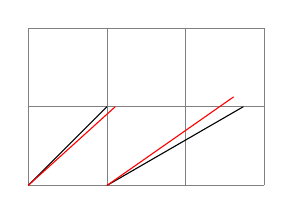
\begin{tikzpicture}
  \draw[style=help lines] (0,0) grid (3,2);
  \draw      (0,0) -- (1,1);
  \draw[red] (0,0) -- ([xshift=3pt] 1,1);
  \draw      (1,0) -- +(30:2cm);
  \draw[red] (1,0) -- +([shift=(135:5pt)] 30:2cm);
\end{tikzpicture}
\end{codeexample}

\subsection{Simple Coordinates}

The simplest way to specify coordinates is as a comma-separated pair
of \TeX\ dimensions as in |(1cm,2pt)| or |(2cm,\textheight)|. As can
be seen, different units can be mixed. The coordinate specified in
this way means ``1cm to the right and 2pt up from the origin of the
picture.'' You can also write things like |(1cm+2pt,2pt)| since the
|calc| package is used. 


\subsection{Polar Coordinates}

You can also specify coordinates in polar coordinates. In this case,
you specify an angle and a distance, separated by a colon as in
|(30:1cm)|. The angle must always be given in degrees and should be
between $-360$ and $720$. 

\begin{codeexample}[]
\tikz \draw    (0cm,0cm) -- (30:1cm) -- (60:1cm) -- (90:1cm)
            -- (120:1cm) -- (150:1cm) -- (180:1cm);
\end{codeexample}

Instead of an angle given as a number you can also use certain
words. For example, |up| is the same as |90|, so that you can write
|\tikz \draw (0,0) -- (2ex,0pt) -- +(up:1ex);|
and get \tikz \draw (0,0) -- (2ex,0pt) -- +(up:1ex);. Apart from |up|
you can use |down|, |left|, |right|, |north|, |south|, |west|, |east|,
|north east|, |north west|, |south east|, |south west|, all of which
have their natural meaning.



\subsection{Xy- and Xyz-Coordinates}

You can specify coordinates in \pgfname's $xy$-coordinate system. In
this case, you provide two unit-free numbers, separated by a comma as
in |(2,-3)|. This means ``add twice the current \pgfname\ $x$-vector and
subtract three times the $y$-vector.'' By default, the $x$-vector
points 1cm to the right, the $y$-vector points 1cm upwards, but this
can be changed arbitrarily using the |x| and~|y| graphic options.

Similarly, you can specify coordinates in the $xyz$-coordinate
system. The only difference to the $xy$-coordinates is that you
specify three numbers separated by commas as in |(1,2,3)|. This is
interpreted as ``once the $x$-vector plus twice the $y$-vector plus
three times the $z$-vector.'' The default $z$-vector points to
$\bigl(-\frac{1}{\sqrt2}
\textrm{cm},-\frac{1}{\sqrt2}\textrm{cm}\bigr)$. Consider the
following example: 

\begin{codeexample}[]
\begin{tikzpicture}[->]
  \draw (0,0,0) -- (1,0,0);
  \draw (0,0,0) -- (0,1,0);
  \draw (0,0,0) -- (0,0,1);
\end{tikzpicture}
\end{codeexample}


\subsection{Node Coordinates}
\label{section-node-coordinates}

In \pgfname\ and in \tikzname\ it is quite easy to define a node that you
wish to reference at a later point. Once you have defined a node,
there are different ways of referencing points of the node.


\subsubsection{Named Anchor Coordinates}

An \emph{anchor coordinate} is a point in a node that you have
previously defined using the node operation. The syntax is
|(|\meta{node name}|.|\meta{anchor}|)|, where \meta{node name} is
the name that was previously used to name the node using the
|name=|\meta{node name} option or the special node name syntax. Here is
an example: 

\begin{codeexample}[]
\begin{tikzpicture}
  \node (shape)   at (0,2)  [draw] {|class Shape|};
  \node (rect)    at (-2,0) [draw] {|class Rectangle|};
  \node (circle)  at (2,0)  [draw] {|class Circle|};
  \node (ellipse) at (6,0)  [draw] {|class Ellipse|};

  \draw (circle.north) |- (0,1);
  \draw (ellipse.north) |- (0,1);
  \draw[-open triangle 90] (rect.north) |- (0,1) -| (shape.south);
\end{tikzpicture}
\end{codeexample}

Section~\ref{section-the-shapes} explain which anchors are available
for the basic shapes. 




\subsubsection{Angle Anchor Coordinates}

In addition to the named anchors, it is possible to use the syntax
\meta{node name}|.|\meta{angle} to name a point of the node's
border. This point is the coordinate where a ray shot from the center
in the given angle hits the border. Here is an example:

\begin{codeexample}[]
\begin{tikzpicture}
  \node (start) [draw,shape=ellipse] {start};
  \foreach \angle in {-90, -80, ..., 90}
    \draw (start.\angle) .. controls +(\angle:1cm) and +(-1,0) .. (2.5,0);
  \end{tikzpicture}
\end{codeexample}


\subsubsection{Anchor-Free Node Coordinates}

It is also possible to just ``leave out'' the anchor and have \tikzname\
calculate an appropriate border position for you. Here is an example:

\begin{codeexample}[]
\begin{tikzpicture}[fill=blue!20]
  \draw[style=help lines] (-1,-2) grid (6,3);
  \path (0,0)  node(a) [ellipse,rotate=10,draw,fill]    {An ellipse}
        (3,-1) node(b) [circle,draw,fill]               {A circle}
        (2,2)  node(c) [rectangle,rotate=20,draw,fill]  {A rectangle}
        (5,2)  node(d) [rectangle,rotate=-30,draw,fill] {Another rectangle};
  \draw[thick] (a) -- (b) -- (c) -- (d);
  \draw[thick,red,->] (a) |- +(1,3) -| (c) |- (b);       
  \draw[thick,blue,<->] (b) .. controls +(right:2cm) and +(down:1cm) .. (d);       
\end{tikzpicture}
\end{codeexample}

\tikzname\ will be reasonably clever at determining the border points that
you ``mean,'' but, naturally, this may fail in some situations. If
\tikzname\ fails to determine an appropriate border point, the center will
be used instead.

Automatic computation of anchors works only with the line-to operations
|--|, the vertical/horizontal versions \verb!|-! and \verb!-|!, and
with the curve-to operation |..|. For other path commands, such as
|parabola| or |plot|, the center will be used. If this is not desired,
you should give a named anchor or an angle anchor.

Note that if you use an automatic coordinate for both the start and
the end of a line-to, as in |--(b)--|, then \emph{two} border
coordinates are computed with a move-to between them. This is usually
exactly what you want.

If you use relative coordinates together with automatic anchor
coordinates, the relative coordinates are always computed relative to
the node's center, not relative to the border point. Here is an
example:

\begin{codeexample}[]
\tikz \draw (0,0) node(x) [draw] {Text}
            rectangle (1,1)
            (x) -- +(1,1);
\end{codeexample}

Similarly, in the following examples both control points are $(1,1)$:

\begin{codeexample}[]
\tikz \draw (0,0) node(x) [draw] {X}
            (2,0) node(y) {Y}
            (x) .. controls +(1,1) and +(-1,1) .. (y);
\end{codeexample}

           
\subsection{Intersection Coordinates}


\subsubsection{Intersection of Two Lines}

Often you wish to specify a point that is on the
intersection of two lines. The first way to specify such an
intersection is the following: You can use the special syntax
\declare{|(intersection of |\meta{$p_1$}|--|\meta{$p_2$}%
  | and |\meta{$q_1$}|--|\meta{$q_2$}|)|}. This will yield the
intersection point of the line going through $p_1$ and $p_2$ and the
line through $q_1$ and $q_2$. If the lines do not meet or if they are
identical and arithmetical overflow error will result.

\begin{codeexample}[]
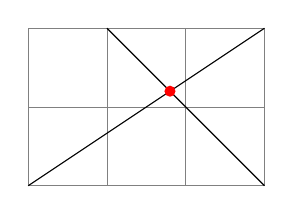
\begin{tikzpicture}
  \draw[help lines] (0,0) grid (3,2);
  \draw (0,0) coordinate (A) -- (3,2) coordinate (B)
        (1,2)                -- (3,0);

  \fill[red] (intersection of A--B and 1,2--3,0) circle (2pt);
\end{tikzpicture}
\end{codeexample}

\subsubsection{Intersection of Horizontal and Vertical Lines}

A frequent special case of intersections is the intersection of a
vertical line going through a point $p$ and a horizontal line going
through some other point $q$. For this situation there is a special,
shorter, syntax: You can say either
\declare{|(|\meta{p}\verb! |- !\meta{q}|)|} or
\declare{|(|\meta{q}\verb! -| !\meta{p}|)|}.

For example, \verb!(2,1 |- 3,4)! and  \verb!(3,4 -| 2,1)! both yield
the same as \verb!(2,4)! (provided the $xy$-coordinate system has not
been modified). 

The most useful application of the syntax is to draw a line up to some
point on a vertical or horizontal line. Here is an example:

\begin{codeexample}[]
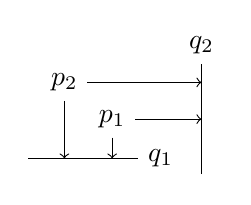
\begin{tikzpicture}
  \path (30:1cm) node(p1) {$p_1$}   (75:1cm) node(p2) {$p_2$};

  \draw (-0.2,0) -- (1.2,0) node(xline)[right] {$q_1$};
  \draw (2,-0.2) -- (2,1.2) node(yline)[above] {$q_2$};

  \draw[->] (p1) -- (p1 |- xline);
  \draw[->] (p2) -- (p2 |- xline);
  \draw[->] (p1) -- (p1 -| yline);
  \draw[->] (p2) -- (p2 -| yline);
\end{tikzpicture}
\end{codeexample}



\subsection{Relative and Incremental Coordinates}

You can prefix coordinates by |++| to make them ``relative.'' A
coordinate such as |++(1cm,0pt)| means ``1cm to the right of the
previous position.'' Relative coordinates are often useful in
``local'' contexts:

\begin{codeexample}[]
\begin{tikzpicture}
  \draw (0,0)     -- ++(1,0) -- ++(0,1) -- ++(-1,0) -- cycle;
  \draw (2,0)     -- ++(1,0) -- ++(0,1) -- ++(-1,0) -- cycle;
  \draw (1.5,1.5) -- ++(1,0) -- ++(0,1) -- ++(-1,0) -- cycle;
\end{tikzpicture}
\end{codeexample}

Instead of |++| you can also use a single |+|. This also specifies a
relative coordinate, but it does not ``update'' the current point for
subsequent usages of relative coordinates. Thus, you can use this
notation to specify numerous points, all relative to the same
``initial'' point:

\begin{codeexample}[]
\begin{tikzpicture}
  \draw (0,0)     -- +(1,0) -- +(1,1) -- +(0,1) -- cycle;
  \draw (2,0)     -- +(1,0) -- +(1,1) -- +(0,1) -- cycle;
  \draw (1.5,1.5) -- +(1,0) -- +(1,1) -- +(0,1) -- cycle;
\end{tikzpicture}
\end{codeexample}

There is one special situation, where relative coordinates are
interpreted differently. If you use a relative coordinate as a control
point of a B�zier curve, the following rule applies: First, a relative
first control point is taken relative to the beginning of the
curve. Second, a relative second control point is taken relative to
the end of the curve. Third, a relative end point of a curve is taken
relative to the start of the curve.

This special behavior makes it easy to specify that a curve should
``leave or arrives from a certain direction'' at the start or end. In
the following example, the curve ``leaves'' at $30^\circ$ and
``arrives'' at $60^\circ$: 

\begin{codeexample}[]
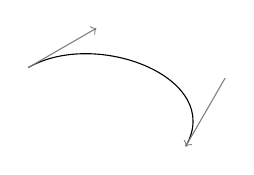
\begin{tikzpicture}
  \draw (1,0) .. controls +(30:1cm) and +(60:1cm) .. (3,-1);
  \draw[gray,->] (1,0) -- +(30:1cm);
  \draw[gray,<-] (3,-1) -- +(60:1cm);
\end{tikzpicture}
\end{codeexample}
